\documentclass[review]{elsarticle}
%-----------------------------------------------------

\usepackage{amsmath}
\usepackage{graphicx}

\graphicspath{{./figs/}}

\newcommand{\ihat}{\boldsymbol{\hat{\textbf{\i}}}}
\newcommand{\jhat}{\boldsymbol{\hat{\textbf{\j}}}}
\newcommand{\roughly}{{\raise.17ex\hbox{$\scriptstyle\sim$}}}
\newcommand{\dmax}{d_\text{max}}
\newcommand{\dmin}{d_\text{min}}

%-----------------------------------------------------

\makeatletter
\renewcommand{\fnum@figure}{Figure 3}
\makeatother

\thispagestyle{empty}

\begin{document}
\allowdisplaybreaks

\begin{figure}[ht]
\centering
%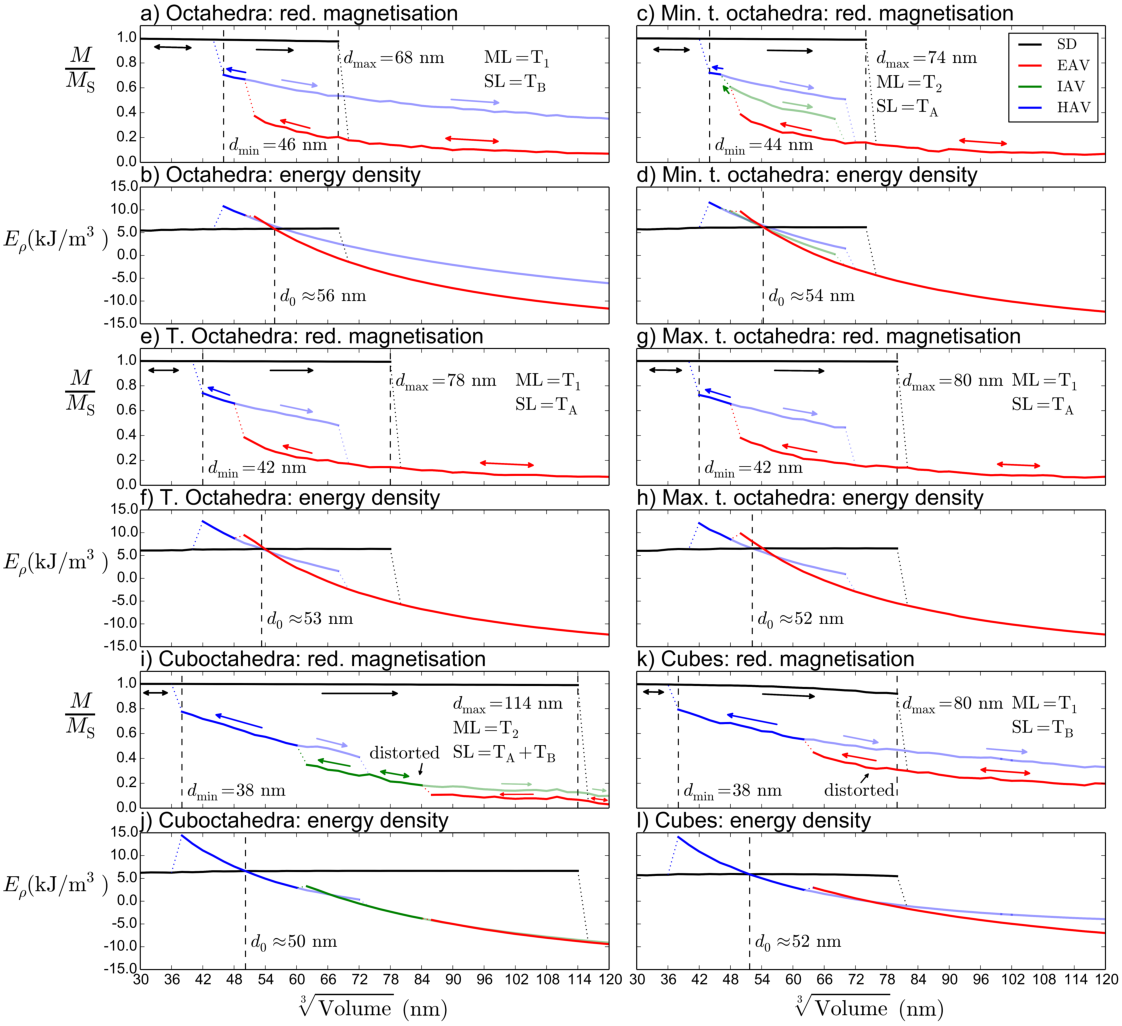
\includegraphics[width=\textwidth]{Figure_03_HR.pdf}
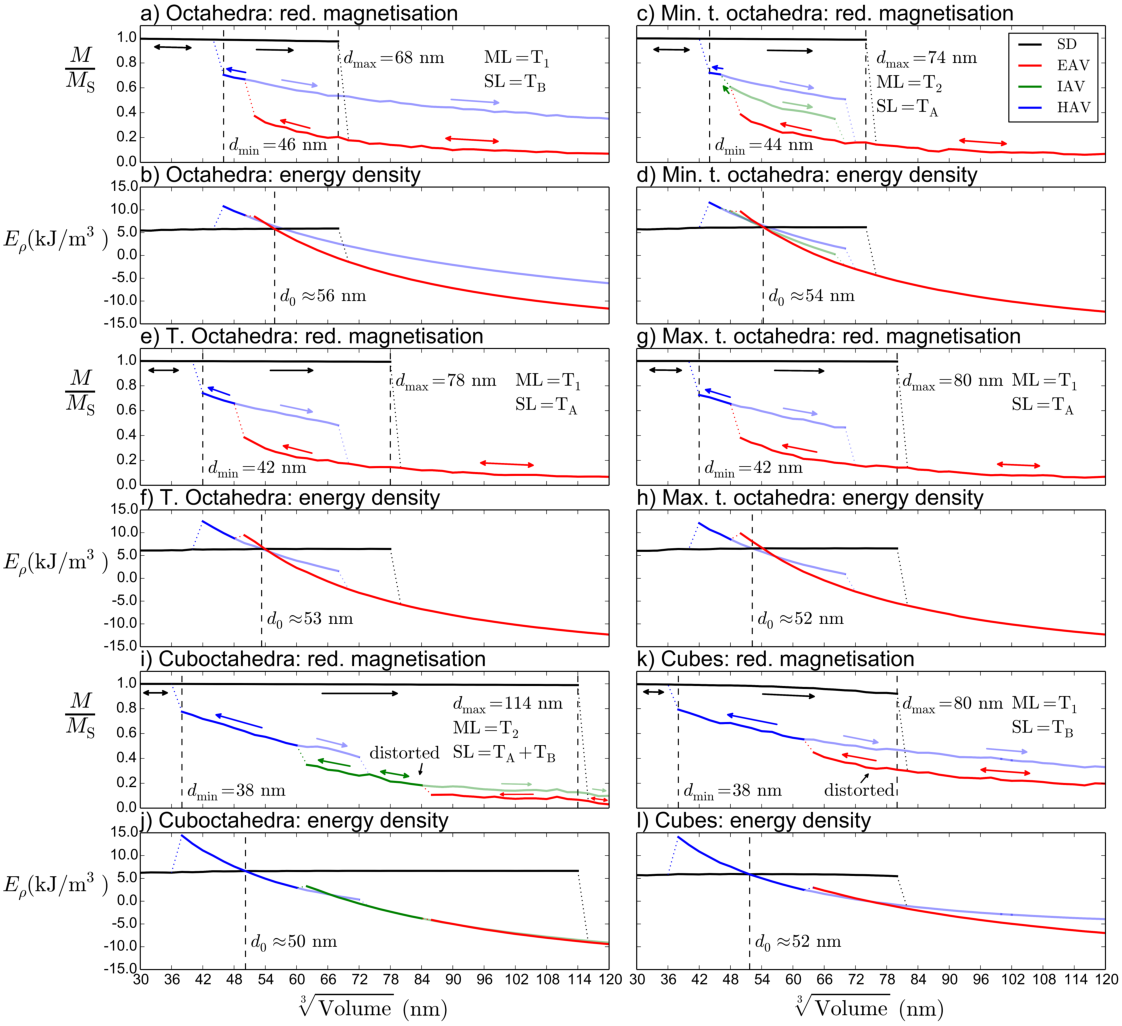
\includegraphics[width=\textwidth]{Figure_03.pdf}
\caption{Domain states and energies in the SD--PSD transition regime. Reduced magnetisation (a, c, e, g, i, k) and energy density (b, d, f, h, j, l) against size. All shapes relax to an easy aligned SD state at 30 nm from a randomised initial condition. The SD state is numerically stable up to $\dmax$ (black lines). Growth beyond $\dmax$ results in the magnetisation relaxing to an EAV, stable up to 120$\,\text{nm}$ (red lines). The solution is then interpolated into smaller grains. This forms the \textit{main loop} (ML) (opaque lines). The EAV is stable down to a threshold beyond which a HAV is nucleated on the size-descending curve. The HAV is stable down to $\dmin$, below which it relaxes to a SD state. This is a Type 1 ML (a, e, g, k). When the EAV goes through an IAV (green lines) before going to the HAV configuration the ML is Type 2 (c, i). Growth of the HAVs and IAVs found on the size-descending curve forms the \textit{secondary loop} (SL) (translucent lines). When these realign with the EAV or with the vortex state they nucleated from the SL is Type A (c, e, g, i (translucent blue line)). When they are stable up to 120$\,\text{nm}$ the SL is Type B (a, i (translucent green line), k).}
\label{fig3}
\end{figure}

\end{document}